%!TEX root = main.tex

\section{Wasm \dslname}
\label{sec:structure}

An overview of Wasm \dslname is illustrated in Figure~\ref{fig:structure}.
%
The Wasm specification is primarily concerned with defining the binary format, type system, and runtime behaviour of Wasm.
%
With \dslname, an author will write these definitions in our \emph{Domain-Specific Language (DSL)}, which the Wasm \dslname toolchain accepts as input.
%
This input is parsed as the \textit{External Language (EL)} representation and processed into further representations,
namely the \textit{Internal Language (IL)} representation,
and the \textit{Algorithmic Language (AL)} representation.
Our various backends use these representations to produce the previously-described output artefacts, as well as \textit{mechanised} definitions in \textit{interactive theorem provers} suitable for machine-checked proofs about the language semantics~\cite{Watt2018MechanisingAV, Watt2021Two}.

As discussed in \cref{sec:intro}, the Wasm specification is currently written in a mixture of
reStructuredText and raw LaTeX.  Figure~\ref{fig:spec} presents the execution
semantics of the $t.\mbox{\emph{binop}}$ binary operator instruction in the Wasm specification~\cite[Section 4.4]{wasm-spec}, as rendered today.
Figure~\ref{fig:spec}(a) shows
the prose pseudocode describing the five execution steps,
and Figure~\ref{fig:spec}(b) shows the mathematics in the gray box for the corresponding
operational semantics.
%
\dslname aims to provide a significantly better developer experience without compromising on the fidelity of the rendered specification.
Moving forward, we will provide a
comprehensive breakdown of each step.

\dslname's DSL and EL are intended to closely mirror an ASCII representation of the syntactic constructs used in Wasm's formal specification.
Figure~\ref{fig:dsl} gives a DSL definition of the runtime semantics of Wasm's binary arithmetic operator,
where {\small\verb!$binop! }is a separately defined auxiliary function.
%
Crucially, all definitions and variables in the parsed EL are ``type-checked'' so that ill-formed definitions can be detected.
For example, if a specification author misses the final argument of 
{\small\verb!$binop!} as in {\small\verb!$binop(binop, nt, c_1)!},
then an arity-mismatch error will be raised.
%
From the EL, \dslname can directly produce the LaTeX-based formal specification, which is intended to replace the current specification's handwritten definitions.
Figure~\ref{fig:latex} is an excerpt from the PDF generated from the LaTeX
translated from Figure~\ref{fig:dsl}.  Compare this to the original handwritten LaTeX in Figure~\ref{fig:spec}.


To produce the other artefacts mentioned in Section~\ref{sec:intro},
the \dslname definitions are processed further.
First, the EL is elaborated into the IL, suitable for deep analysis and transformation.
Among other things, types and multiplicities of variables are inferred and annotated in the IL, mutually recursive definitions are identified, and implicit upcasts are made explicit and disambiguated.
%
As Figure~\ref{fig:structure} illustrates, the IL can undergo internal transformations to meet the needs of subsequent backends.
%
For example, in the EL expressions are modelled as
relations that can fail or can denote multiple values,  whereas various theorem prover
backends require that expressions must be purely functional, i.e.\ must denote exactly
one value given values for all free variables.
Figure~\ref{fig:lean} is an excerpt from the code generated for the Lean theorem prover~\cite{Moura2015TheLT}.
We are currently working on similarly generating code for Coq, Isabelle, and Agda.

The operational semantics of Wasm described in the IL is further transformed into the more restricted AL,
which does not allow arbitrary relational definitions and
enforces an algorithmic order of evaluation.
The problem of transforming a relational definition into an
executable, algorithmic one is known as \textit{animation}~\cite{animate}.
At its core, the process of animation involves performing a dataflow analysis on a relational definition to infer which equations of the relational definition should be interpreted as binding new variables, and ensures that these binding definitions can be ordered such that each binding definition only depends on prior animated definitions.

%!TEX root = ../main.tex

\begin{figure}[t]
  \centering
  \begin{subfigure}{\columnwidth}
    \centering
    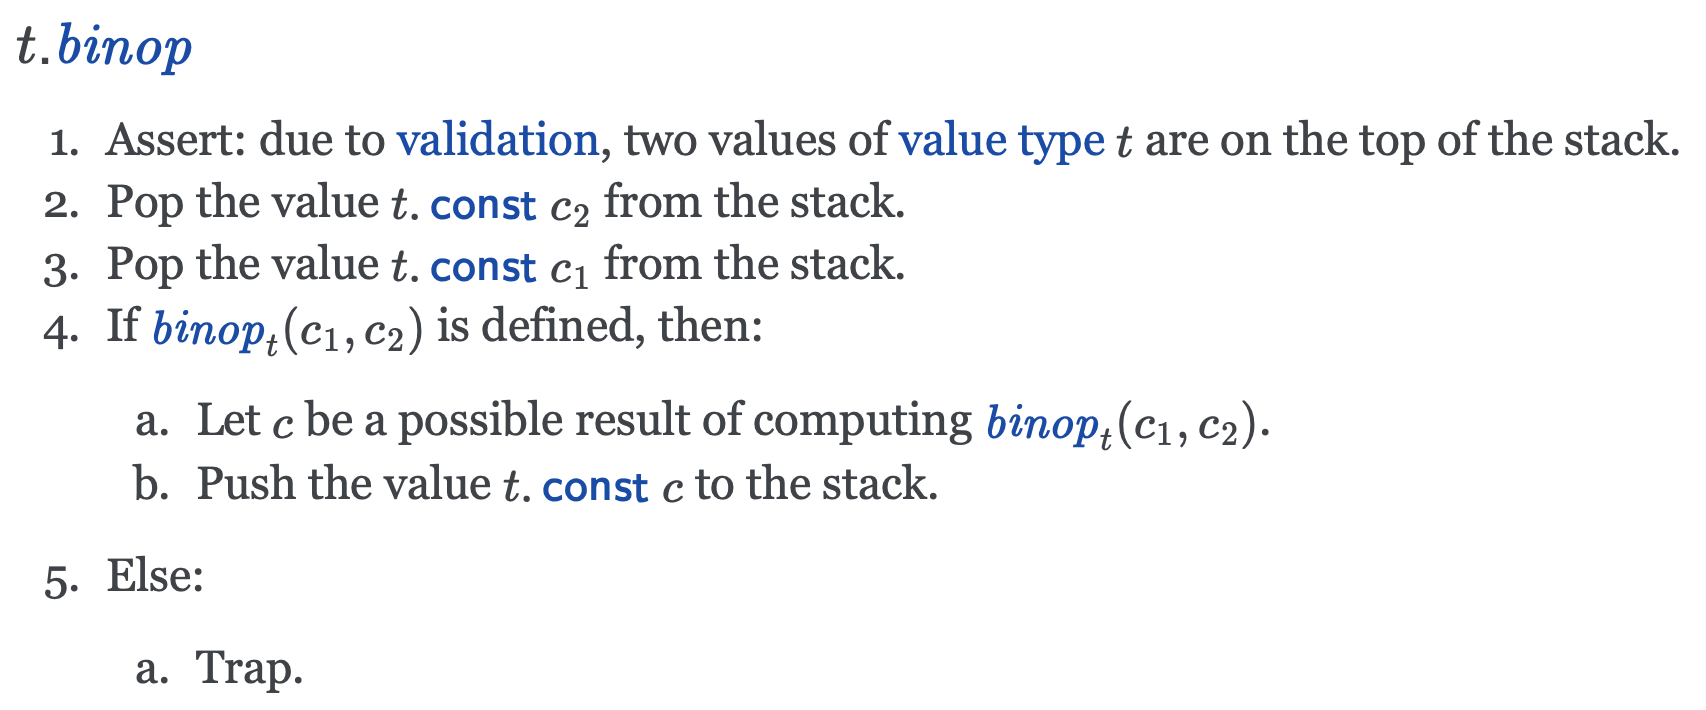
\includegraphics[width=\columnwidth]{figs/spec-prose.png}
    \subcaption{Prose specification}
\vspace*{1em}
  \end{subfigure}

  \begin{subfigure}{\columnwidth}
    \centering
    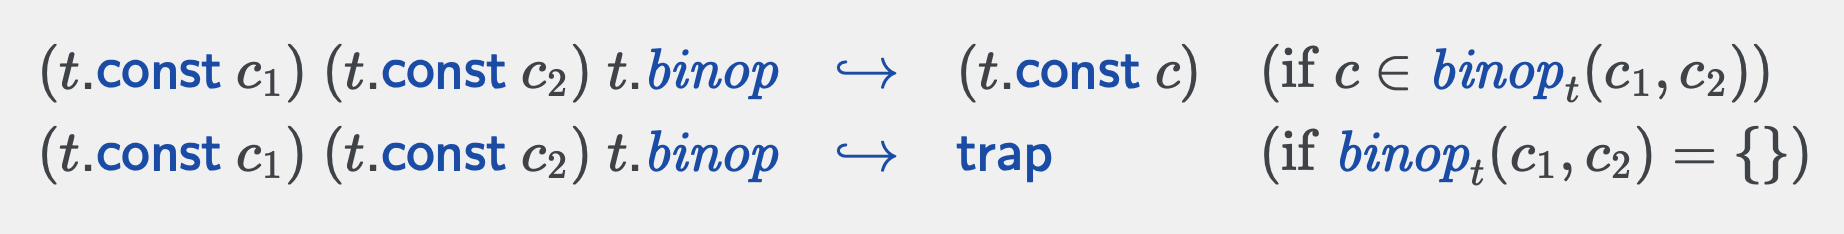
\includegraphics[width=\columnwidth]{figs/spec-formal.png}
    \subcaption{Formal specification}
  \end{subfigure}
\caption{The binary operator semantics in the specification}
\label{fig:spec}
\end{figure}

\begin{figure}[t]
\small
\begin{verbatim}
rule Step_pure/binop-val:
  (CONST nt c_1) (CONST nt c_2) (BINOP nt binop) ~> (CONST nt c)
  -- if $binop(binop, nt, c_1, c_2) = c

rule Step_pure/binop-trap:
  (CONST nt c_1) (CONST nt c_2) (BINOP nt binop) ~> TRAP
  -- if $binop(binop, nt, c_1, c_2) = epsilon
\end{verbatim}
\caption{The binary operator semantics in \dslname's DSL}
\label{fig:dsl}
\end{figure}

\begin{figure}[t]
\small
$$
\begin{array}{@{}l@{}lcl}
{[\textsc{\scriptsize E{-}binop{-}val}]} \ \
 & (\mathit{nt}.\mathsf{const}~\mathit{c}_{1})~(\mathit{nt}.\mathsf{const}~\mathit{c}_{2})~(\mathit{nt} . \mathit{binop})
 &\hookrightarrow& (\mathit{nt}.\mathsf{const}~\mathit{c}) \\
%
& \mbox{if}~{{{\mathit{binop}}{}}_{\mathit{nt}}}{(\mathit{c}_{1},\, \mathit{c}_{2})} = \mathit{c} \\
%
{[\textsc{\scriptsize E{-}binop{-}trap}]} \ \
 & (\mathit{nt}.\mathsf{const}~\mathit{c}_{1})~(\mathit{nt}.\mathsf{const}~\mathit{c}_{2})~(\mathit{nt} . \mathit{binop})
 &\hookrightarrow& \mathsf{trap} \\
%
& \mbox{if}~{{{\mathit{binop}}{}}_{\mathit{nt}}}{(\mathit{c}_{1},\, \mathit{c}_{2})} = \epsilon
\end{array}
$$
\vspace*{-1em}
\caption{The binary operator semantics in a generated PDF}
\label{fig:latex}
\end{figure}

\begin{figure}[t]
\footnotesize
\begin{verbatim}
  | binop_val  (binop : Binop_numtype) (c : C_numtype) (c_1 : C_numtype)
               (c_2 : C_numtype) (nt : Numtype) : 
    ((«$binop» (binop, nt, c_1, c_2)) == [c]) -> 
    (Step_pure ([(Admininstr.CONST (nt, c_1)),
                 (Admininstr.CONST (nt, c_2)),
                 (Admininstr.BINOP (nt, binop))],
                [(Admininstr.CONST (nt, c))]))

  | binop_trap (binop : Binop_numtype) (c_1 : C_numtype)
               (c_2 : C_numtype) (nt : Numtype) : 
    ((«$binop» (binop, nt, c_1, c_2)) == []) -> 
    (Step_pure ([(Admininstr.CONST (nt, c_1)),
                 (Admininstr.CONST (nt, c_2)),
                 (Admininstr.BINOP (nt, binop))],
                [Admininstr.TRAP]))
\end{verbatim}
\caption{The binary operator semantics in generated Lean}
\label{fig:lean}
\end{figure}

{\sloppypar
Figure~\ref{fig:al} shows how the declarative specification of the
binary operator semantics from Figure~\ref{fig:dsl} is translated to the algorithmic version.
Note that the implicit conditions guaranteed by the Wasm validation phase
are explicitly added as assertions such as
{\small\verb!AssertI(TopValueC(NameE(nt)))!}.
Interestingly, two equality expressions are translated to different AL constructs.
Because the equality ``{\small\verb!if $binop(binop, nt, c_1, c_2) = c!}'' is a binding
that binds the result of the {\small\verb!$binop!} call to {\small\verb!c!}, it is translated as
a {\small\verb!let!} instruction:
}

\smallskip
{\small
\begin{verbatim}
    LetI(ListE([NameE(c)]),
         AppE(binop, [NameE(binop), NameE(nt),
                      NameE(c_1), NameE(c_2)]))
\end{verbatim}
}
\smallskip

\noindent
On the contrary, since ``{\small\verb!if $binop(binop, nt, c_1, c_2) = epsilon!}''
is an equality check which is inferred to bind no new variable, it is translated as a conditional expression:

\smallskip
{\small
\begin{verbatim}
    CompareC(is, AppE(binop, [NameE(binop), NameE(nt),
                              NameE(c_1), NameE(c_2)]),
             ListE([]))
\end{verbatim}
}
\smallskip

\begin{figure}[t]
\footnotesize
\begin{verbatim}
execution_of_BINOP_ainstr NameE(nt) NameE(binop):
  AssertI(TopValueC(NameE(nt)))
  PopI(ConstructE(CONST_ainstr, [NameE(nt), NameE(c_2)]))
  AssertI(TopValueC(NameE(nt)))
  PopI(ConstructE(CONST_ainstr, [NameE(nt), NameE(c_1)]))
  IfI(
    CompareC(is, LengthE(AppE(binop, [NameE(binop), NameE(nt),
                                      NameE(c_1), NameE(c_2)])), 1),
    [LetI(ListE([NameE(c)]),
          AppE(binop, [NameE(binop), NameE(nt),
                       NameE(c_1), NameE(c_2)]))
     PushI(ConstructE(CONST_ainstr, [NameE(nt), NameE(c)]))],
    [])
  IfI(
    CompareC(is, AppE(binop, [NameE(binop), NameE(nt),
                              NameE(c_1), NameE(c_2)]), ListE([])),
    [TrapI],
    [])
\end{verbatim}
\caption{The binary operator semantics in \dslname's AL}
\label{fig:al}
\end{figure}


From the AL, we directly generate a prose pseudocode specification.
Figure~\ref{fig:gen-spec} shows the prose pseudocode generated from the specification in Figure~\ref{fig:al},
which is strikingly close to the original handwritten prose description in Figure~\ref{fig:spec}.
%
We also implement an interpreter for the AL.
%
By interpreting AL that represents the Wasm semantics, we indirectly obtain an interpreter for Wasm.
%
This technique was previously used by JISET~\cite{jiset,esmeta}
to extract an executable semantics from the ECMAScript prose that represents the official
JavaScript specification~\cite{ecmascript}, and we use it here to extract an executable semantics for Wasm, from the \dslname AL.

Currently, Wasm \dslname covers all of Wasm 2.0 except for the recently-standardized SIMD vector instructions.
Within one second, our toolchain can automatically generate both prose pseudocode and operational semantics in LaTeX
with hyperlinks and cross-references in the generated PDF document, and a Lean mechanization.
We tested the extracted Wasm semantics against the official Wasm unit test suite
on an Ubuntu machine with
a 4.0GHz Intel(R) Core(TM) i7-6700k and 32GB of RAM (Samsung DDR4 2133MHz 8GB*4).
On this machine, the extracted semantics passed all 23,778 tests (SIMD excluded) in the
test suite in 21.349 seconds.

\begin{figure}[t]
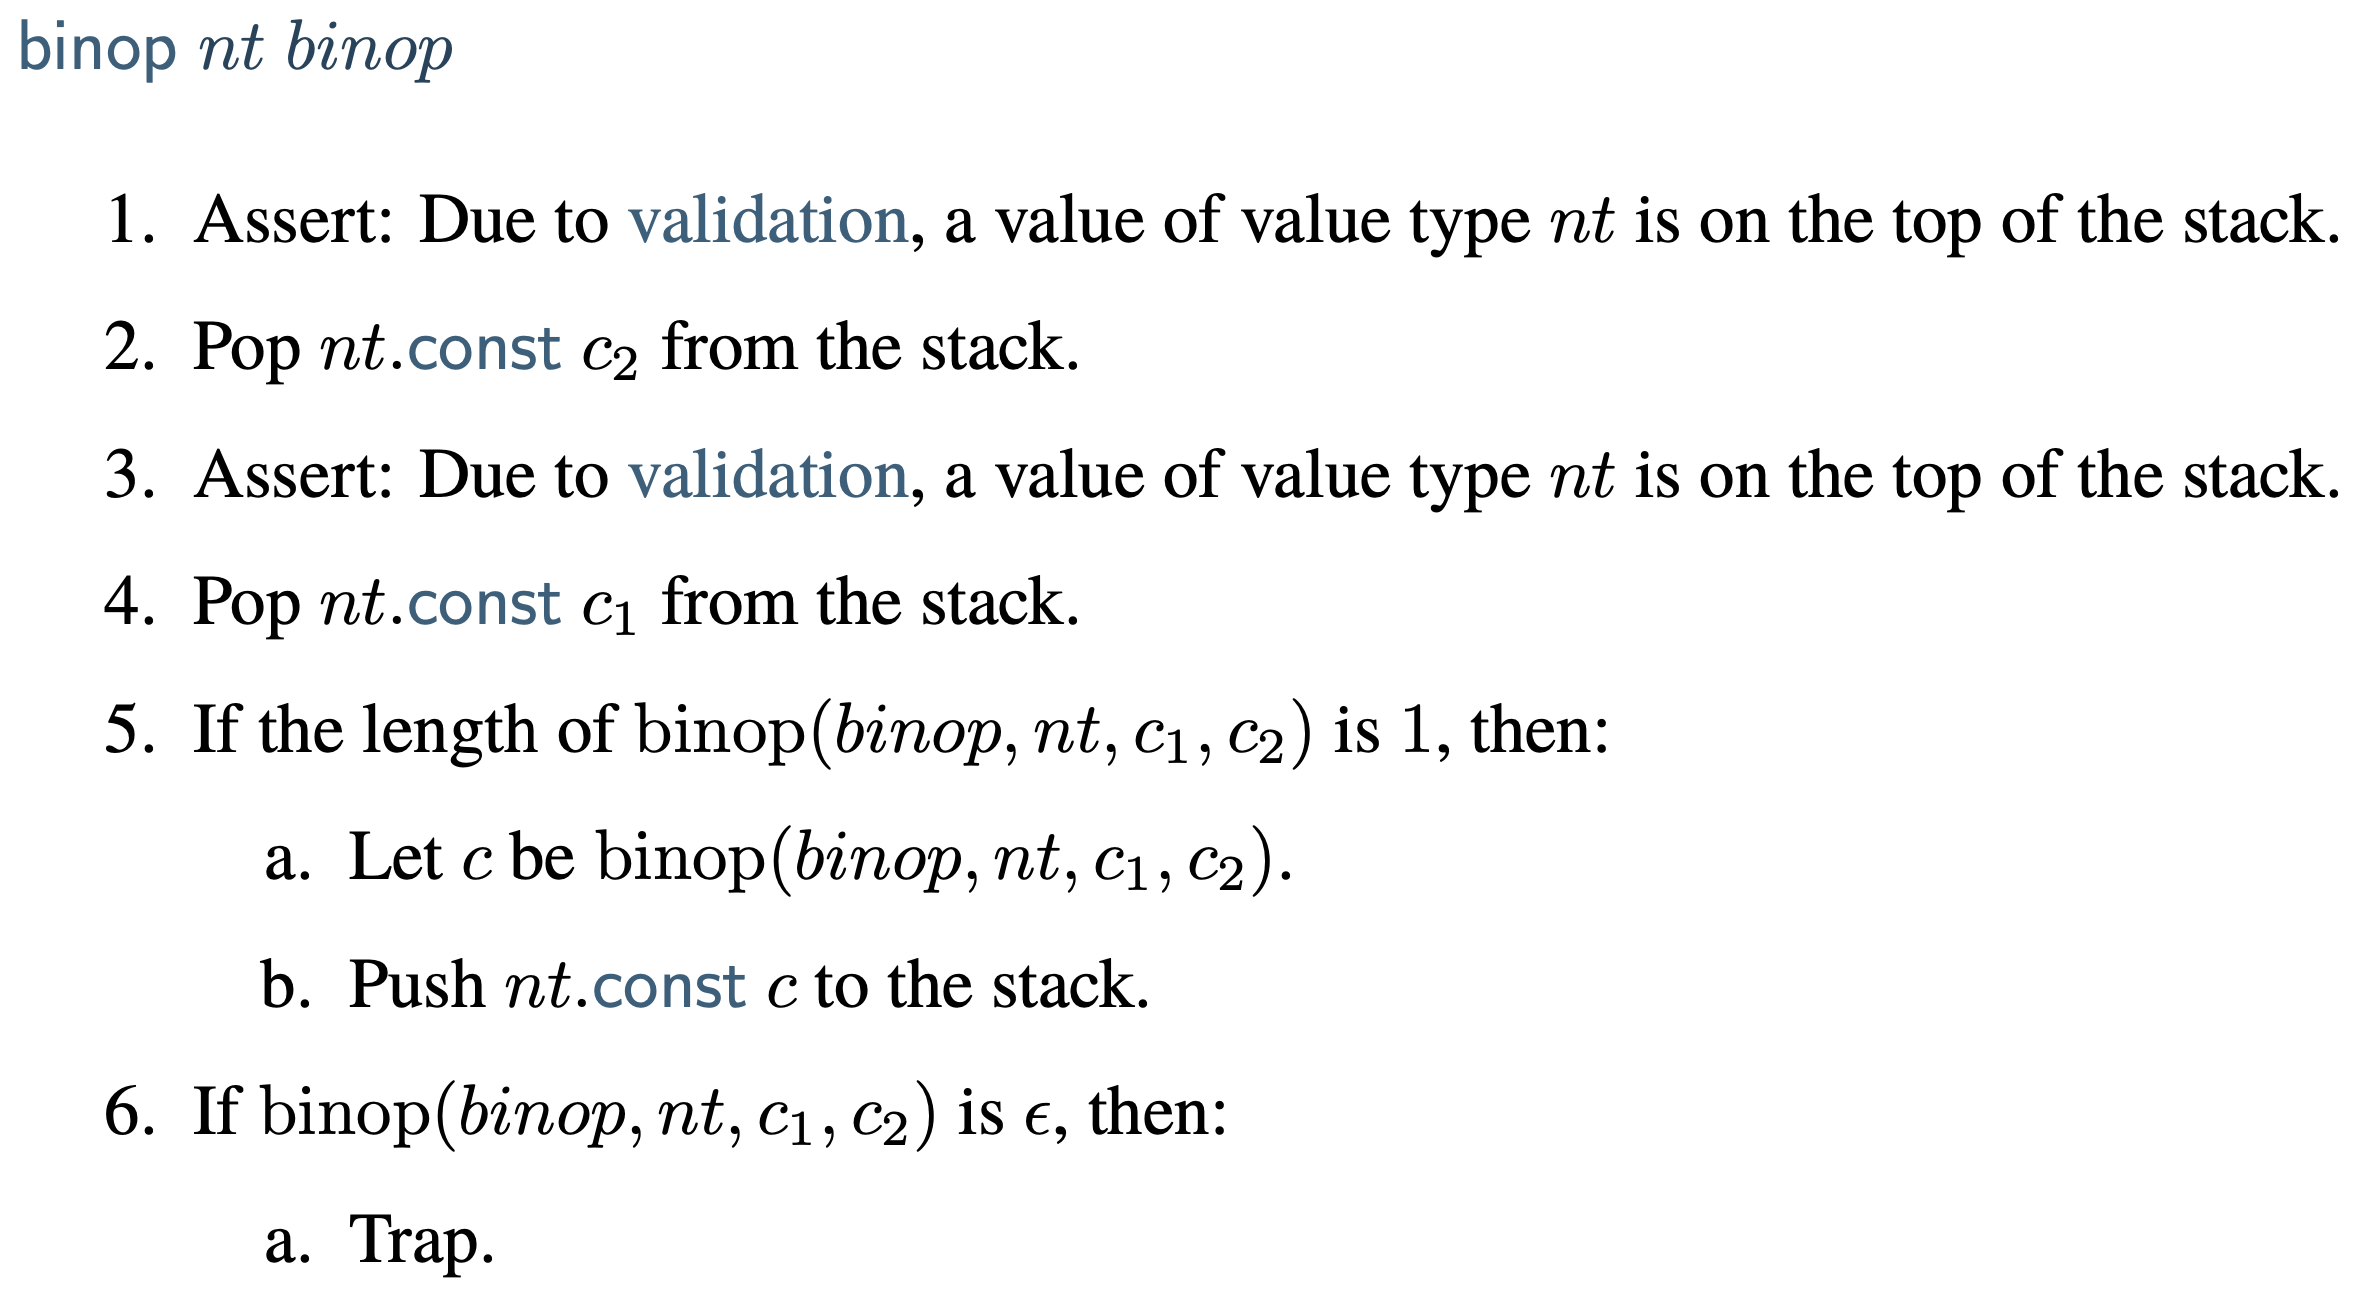
\includegraphics[width=.48\textwidth]{figs/gen-spec.png}
\caption{The binary operator semantics in generated prose}
\label{fig:gen-spec}
\end{figure}
